\begin{figure}[!t!h!b!]
\centering
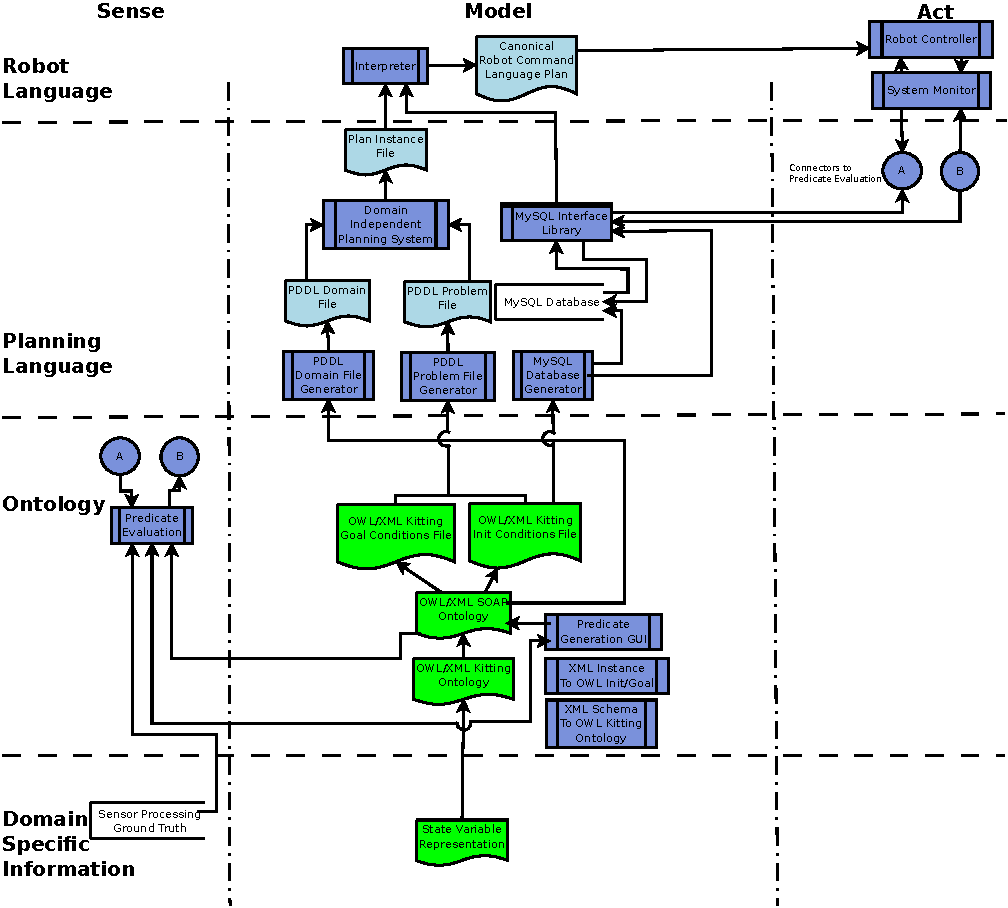
\includegraphics[width=10cm]{images/KnowledgeDrivenRobotics.pdf}
\caption{Knowledge Driven Design extensions -- In this figure, green shaded
  boxes with curved bottoms represent hand generated files while light blue
  shaded boxes with curved bottoms represent automatically created boxes.
  Rectangular boxes represent processes and libraries. }
\label{fig:methodology}
\end{figure}


The knowledge driven methodology presented in this section is not intended to act as a stand-alone system architecture. Rather it is intended to be an extension to well developed hierarchical, deliberative architectures such as 4D/RCS (Real-time Control Systems)~\cite{Albus2000}. The overall knowledge driven methodology of the system is depicted in Figure~\ref{fig:methodology}. The figure is organized vertically by the representation that is used for the knowledge and horizontally by the classical sense-model-act paradigm of intelligent systems. The remainder of this section gives a brief description of each level of the hierarchy to help the reader understand the basic concepts implemented within the system architecture in order that the reader may better grasp the main effort described in this paper. The reader may find a more detailed description of each component and each level of the architecture in other publications~\cite{BALAKIRSKY.IROS.2012}.

\subsection{Domain Specific Information}
\label{subsection:DSI}
On the vertical axis, knowledge begins with Domain Specific Information (DSI). DSI includes sensors and sensor processing that are specifically tuned to operate in the target domain. Examples of sensor processing may include pose determination and object identification. It is important to note that the effort described in this paper assumes perfect data from the sensor system that do not include noise. A detailed description of the simulated sensor system is given in Section~\ref{sect:simulation}.

For the knowledge model, a scenario driven approach is taken where the DSI design begins with a domain expert creating one or more use cases and specific scenarios that describe the typical operation of the system. This includes information on items ranging from what actions and attributes are relevant, to what the necessary conditions (preconditions) are for an action to occur and what the likely results (effects) of the action are. The authors have chosen to encode this basic information in a formalism known as a state variable representation~\cite{NAU.2004}.


% Based on the action description, objects in the environment that are relevant for system operation can be identified. For example, the action \textsf{take-part}, depicted in Figure 2, has a given robot place a kit tray onto a work table. The preconditions for this action are that the robot is holding a kit tray and there is a clear space on the table to place the tray. This is represented by the predicate expressions shown in Figure 2 that specify that the robot is holding the kit tray, the kit tray is located on the robot (actually in its  gripper), and the work table is empty. The expected effects of this action are that the kit tray is now located on the work table and the robot is no longer holding it. This is also represented by a series of predicates that are shown in Figure 2. Based on the preconditions and expected effects, the objects that are relevant to this action include the robot, the kit tray, and the work table. Aspects of these items may now be represented in the DSI. For example, that a
kit tray has a location and may be held by the robot or placed on the work table.

\subsection{Ontology}
\label{subsection:ontology}
The information encoded in the DSI is then organized into a domain
independent representation.

\begin{itemize}
\item A base ontology (\textsf{OWL/XML Kitting})
contains all of the basic information that was determined to be needed
during the evaluation of the use cases and scenarios. The knowledge is
represented in a compact form with knowledge classes
inheriting common attributes from parent classes.
\item The \textsf{OWL/XML SOAP} ontology describes the links between States, Ordering constructs, Actions, and Predicates (the SOAP
ontology) that are relevant to the scenario. A State is composed of one to many state relationships, which is
a specific relation between two objects (e.g., Object 1 is on top of Object 2). An Ordering construct defines the order in which the state relationships need to be
represented for a specific State. In classical representation, States are represented as sets of logical
atoms (Predicates) that are true or false within some interpretation. Actions are represented by
planning operators that change the truth values of these atoms. In the case of the kit building domain, it was found that 10 actions and
16 predicates were necessary.

\item The instance files describe the initial and goal states for the
system through the \textsf{Kitting Init Conditions File} and the
\textsf{Kitting Goal Conditions File}, respectively. The initial state file
must contain a description of the environment that is complete enough for a
planning system to be able to create a valid sequence of actions that will
achieve the given goal state. The goal state file only needs to contain
information that is relevant to the end goal of the system. For the case of building a kit, this may simply be that a complete kit is located in a bin designed to hold completed kits.

\end{itemize}




%The \textsf{OWL/XML SOAP} ontology describes not only aspects of actions and predicates but also the
%individual actions and predicates that are necessary for the domain under study.



%
% <<<<<<< HEAD
% Since both the OWL (Web Ontology Language) \cite{OWLoverview} and XML implementations of the knowledge representation are file based, real-time information proved to be problematic. In order to solve this problem, an automatically generated MySQL database has been introduced as part of the knowledge representation.
% While the knowledge representation presented in this paper provides the \lq\lq{}slots\rq\rq{} necessary for representing dynamic information, the
% static file structure makes the utilization of these slots awkward. It is desirable to be able to represent the dynamic information in a dynamic database. For this reason, the authors have developed a technique for automatically generating tables for storing,  and access functions for obtaining, the data from the ontology in a MySQL database.
%
% Reading data from and to the MySQL database instead of the ontology file offers the community easy access to a live data structure. Furthermore, it is more practical to modify the information stored in a database than if it was stored in an ontology, which in some cases, requires the deletion and re-creation of the whole file. A literature review reveals many efforts and methodologies that have been designed to produce SQL databases from ontologies. Our effort builds upon the work of Astrova et al.\cite{Astrova2007}.
%
% In addition to generating and filling the database tables, the authors have created tools that automatically generate a set of C{}\texttt{++} classes for reading and writing
% information to the kitting MySQL database. The choice of C{}\texttt{++} was a team preference and we believe that other object-oriented languages could have been used in this project.
%
% The interaction of the MySQL database with the Connectors to Predicate Evaluation (in the Act level) is detailed in Section \ref{sec:sensor-1}.
%
% =======
Since both the OWL and XML implementations of the knowledge representation are file based, real time information proved to be problematic. In order to solve this problem, an automatically generated \textsf{MySQL Database} \cite{MySQL} has been introduced as part of the knowledge representation. A description of the \textsf{MySQL Database} is given in the following subsection.


%
%The Generator tool is a graphical user interface developed in Java, allowing the user to store data from OWL files into a MySQL database. This tool also permits the user to query the database using the C++ function calls. The tool Generator is composed of the following functionalities:
%\begin{enumerate}
% \item Convert OWL documents into SQL syntax (OWL to SQL).
% \item Translate SQL syntax to OWL language in order to modify an OWL document (SQL to OWL).
% \item Convert the OWL language into C++ classes (OWL to C++).
%\end{enumerate}
%
%To date, only steps 1. and 3. have been implemented and will be covered in this document.
%In order to generate the SQL database and C++ classes, the OWL object model must be mapped to the C++ object model and the relational SQL model.
%To quote the OWL 2 Web Ontology website~\cite{OWLspec}, ``Entities are the fundamental building blocks of OWL 2 ontologies,
%and they define the vocabulary --the named terms-- of an ontology. In logic, the set of entities is usually said to constitute the
%signature of an ontology''. Therefore, the notions of single-valued and multi-valued properties as well as the inheritance must be
%mapped from the ontology to the SQL database and C++ classes. The mapping from OWL proceeds as follows:
%\begin{itemize}
%\item Data properties: In an ontology, data properties link an individual to a data value. Single-valued data properties are mapped into a SQL table entry or C++ class
%variable with the corresponding type of the original property. For example, in the ontology a robot has a single-valued data
%property \texttt{hasRobot\_Description}, represented in the
%SQL database as a \texttt{varchar} and in the corresponding C++ class as \texttt{std:string}.
%Multi-valued data properties are mapped from the ontology into the SQL database as a table and into the C++ class as a \texttt{std:vector} with the corresponding
%type of the original property. For example,
%in the ontology a stock keeping unit has a multi-valued
%data property \texttt{hasSku\_EndEffectorRefs}. This maps to a SQL table containing \texttt{varchar} entries and the C++
%\texttt{std::vector\textless std::string\textgreater} in the corresponding C++ class.
%
%\item Object property: In an ontology, object properties link one individual to another individual.
%The single-valued object properties are mapped to a SQL table entry or C++ class
%variable. Their type is a pointer to the range of the object properties. For example, in the ontology a solid object has the object property \texttt{hasRobot\_Description}
%linking it to a physical location. In the SQL database, we use a foreign key to link the two entries. In the C++ classes, this is represented by a reference to a physical location: \texttt{PhysicalLocation* hasSolidObject\_PrimaryLocation}.
%Multi-valued object properties are mapped from the ontology into the SQL database as a table and into the C++ class as a \texttt{std:vector} of pointers referencing objects of the range of the property.  For example, a solid object also has a list of secondary locations corresponding to a multi-valued object property in the ontology:\\ \texttt{std::vector\\ \textless PhysicalLocation*\textgreater hasSolidObject\_SecondaryLocation}.
%\end{itemize}


\subsection{Planning Language}
\label{subsection:planning_language}
Aspects of the knowledge previously described are automatically extracted and encoded in a form that is optimized for a planning system to utilize (the Planning Language). The planning language used in the knowledge driven system is expressed with the Planning Domain Definition Language (PDDL)~\cite{PDDL} (version 3.0). The PDDL input format consists of two files that specify the domain and the problem. As shown in Figure~\ref{fig:methodology}, these files are automatically generated from the ontology. From these two files, a domain independent planning system~\cite{Coles.ICAPS.2010} was used to produce a static \textsf{Plan Instance File}.



While the knowledge representation presented in this paper provides the \lq\lq{}slots\rq\rq{} necessary for representing dynamic information, the
static file structure makes the utilization of these slots awkward. It is desirable to be able to represent the dynamic information in a dynamic database.
For this reason, the authors have developed a technique to automatically generate tables for storing, and access functions
for obtaining the data from the ontology in a \textsf{MySQL Database}.

Reading data from and to the \textsf{MySQL Database} instead of the ontology file offers the community easy access to a live data structure. Furthermore, it is more practical to modify the information stored in a database than if it was stored in an ontology, which in some cases, requires the deletion and re-creation of the whole file. A literature review reveals many efforts and methodologies that have been designed to produce SQL databases from ontologies. Our effort builds upon the work of Astrova \textit{et al.} \cite{Astrova2007}

In addition to generating and filling the database tables, the authors have created tools that automatically generate a set of C{}\texttt{++} classes for reading and writing
information to the kitting \textsf{MySQL Database}. The choice of C{}\texttt{++} was a team preference and we believe that other object-oriented languages could have been used in this project.

\subsection{Robot Language}
\label{subsection:robot_language}
Once a plan has been formulated, the knowledge is transformed into a representation that is optimized for use by a robotic system. The interpreter combines knowledge from the plan with knowledge from the \textsf{MySQL Database} to form a sequence of sequential actions that the robot controller is able to execute. The authors devised a canonical robot command language (CRCL) in which such lists can be written. The purpose of the CRCL is to provide generic commands that implement the functionality of typical industrial robots without being specific either to the language of the planning system that makes a plan or to the language used by a robot controller that executes a plan. 